\documentclass[12pt]{ctexart}
\usepackage{amsmath,graphicx,textcomp,subfigure,indentfirst,ctex,color,float}
\usepackage{bm, mhchem}
\usepackage{framed}
\usepackage{xcolor}
\colorlet{shadecolor}{orange!15}
\title{Lecture 11}
\author{授课、校对:茅奕  \\ 记录:赵思逸}

\date{\today}
\newcommand{\new}[1]{\textcolor{blue}{#1}}

\newcommand{\refeq}[1]{式~(\ref{#1})}
\newcommand{\refeqs}[2]{式~(\ref{#1}) - (\ref{#2})}
\newcommand{\reffig}[1]{图~(\ref{#1})}

\begin{document}

\maketitle

本课程星系部分将讨论线性微扰理论、非线性结构的形成、暗物质晕结构、盘星系的形成、椭圆星系的形成。

\section{线性微扰理论}

本节考虑线性结构,即 $\frac{\delta \rho}{\rho} \ll 1$.

我们将重子物质和光子辐射视为流体,考虑
流体的演化方程。
流体的主要性质有 密度 $\rho\left(\vec{r},t\right) $ 、速度 $\vec{u}\left(\vec{r},t\right) $ 、压强 $P\left(\vec{r},t\right) $   。其中 $\vec{r}$ 是物理坐标系(proper coordinates)中的位置。

\subsection{流体演化方程}
流体满足以下三个方程: 

\subsubsection*{连续性方程}

连续性方程来自能量守恒,描述局域密度的变化。
\begin{equation}
    \frac{\partial \rho}{\partial t} + \nabla \cdot \left(\rho \vec{u}\right) = 0
\end{equation}

将括号中写开得到
\begin{equation}
    \frac{\partial \rho}{\partial t} + \vec{u}\cdot \nabla \rho + \rho \nabla \cdot \vec{u} = 0
\end{equation}

定义拉格朗日导数
\begin{equation}
    \frac{D}{D t} = \left.\frac{\partial}{\partial t} \right|_{\vec{r}} + \vec{u}\cdot \nabla_{\vec{r}}
\end{equation}
其中第一项 $\left.\frac{\partial}{\partial t} \right|_{\vec{r}}$ 是欧拉导数(Eulerian derivative),第二项来自流体的运动 $\vec{u}\cdot \nabla_{\vec{r}} = \frac{\partial \vec{r}}{\partial t} \cdot \left.\frac{\partial}{\partial \vec{r}}\right|_t$.

则连续性方程变成
\begin{equation} \label{eq:continu}
    \frac{D \rho}{D t} + \rho \nabla_{\vec{r}} \cdot \vec{u} = 0
\end{equation}

\subsubsection*{欧拉方程}

定义引力势 $\phi$. 欧拉方程是
\begin{equation}
    \frac{D \vec{u}}{D t} = -\frac{\nabla_{\vec{r}} P}{\rho} - \nabla_{\vec{r}} \phi
\end{equation}
欧拉方程描述流体的运动,其中第一项由压强的梯度贡献,第二项由引力势贡献。

\subsubsection*{泊松方程}

泊松方程描述引力势和密度的关系。
\begin{equation} \label{eq:Poisson}
    \nabla_{\vec{r}}^2 \phi = 4\pi G \rho
\end{equation}

现在我们有 $\left(\rho, u_{i}, u_{j}, u_{k}, P, \phi\right)$ 6个未知量,5个方程(其中欧拉方程是矢量方程,相当于三个分量各有一个方程),需要引入物态方程 $P=P\left(\rho\right)$ 后才能解。

\subsection{共动坐标系下的方程}
在膨胀宇宙中,为了方便计算,我们采取共动坐标系,记共动坐标为 $\vec{x}$,共动坐标系下的物理量与物理坐标系下的物理量有以下关系
\begin{eqnarray}
    \vec{r} &=& a(t) \vec{x} \label{eq:como_r}\\ 
    \vec{u} &=& \dot{a}(t) \vec{x} + \vec{v} \\ 
    \left.\nabla_{\vec{r}}\right|_t &=& \frac{1}{a(t)} \nabla_{\vec{x}} \\ 
    \left. \frac{\partial}{\partial t} \right|_{\vec{r}} &=& \left. \frac{\partial}{\partial t} \right|_{\vec{x}} + \frac{\partial \vec{x}}{\partial t} \bigg|_{\vec{r}} \cdot \nabla_{\vec{x}} = \frac{\partial}{\partial t} \bigg|_{\vec{x}} - \frac{\dot{a}}{a} \vec{x} \cdot \nabla_{\vec{x}}
\end{eqnarray}
其中$\vec{v} \equiv a(t) \dot{\vec{x}}$是本动速度,
以下我们省略下标$\vec{x}$.

将密度改写成平均密度和涨落(fluctuations)的形式
\begin{equation}
    \rho \left(\vec{x},t\right) = \bar{\rho}\left(t\right)  \left[1+\delta \left(\vec{x}, t\right) \right] 
\end{equation}
其中 $\delta \left(\vec{x}, t\right)$ 称为涨落或起伏(fluctuations).
对于重子物质,有 
\begin{equation} \label{eq:a-3}
    \bar{\rho}\propto a^{-3}
\end{equation}

将 \refeqs{eq:como_r}{eq:a-3} 代入\refeqs{eq:continu}{eq:Poisson},得到:

连续性方程
\begin{equation}
    \frac{\partial \delta}{\partial t}+\frac{1}{a} \nabla \cdot[(1+\delta) \vec{v}]=0
\end{equation}

欧拉方程
\begin{equation} \label{eq:Euler-como}
    \frac{\partial \vec{v}}{\partial t}+\frac{\dot{a}}{a} \vec{v}+\frac{1}{a}(\vec{v} \cdot \nabla) \vec{v}=-\frac{\nabla P}{a \bar{\rho}(1+\delta)}-\frac{\nabla \Phi}{a}
\end{equation}

% 密度涨落和熵涨落都会影响

泊松方程
\begin{equation} \label{eq:Poisson-como}
    \nabla^{2} \Phi=4 \pi G \bar{\rho} a^{2} \delta
\end{equation}
其中 $\Phi = \phi + \frac{a \ddot{a} \vec{x}^2}{2}$ 是修正引力势(modified gravitational potential)。

改写到共动坐标系后我们还是有 6个未知量 $\left(\rho, \vec{v}, P, \Phi\right)$ ,5个方程,需要引入物态方程 $P=P\left(\rho, T\right)$ 或 $P=P\left(\rho,  S\right)$ 后才能解。

\subsection{理想气体状态方程}

我们考虑重子气体,单原子气体(比如原子氢、氦气体)的理想气体状态方程
\begin{equation}
    P=nk_BT =\frac{\rho}{\mu m_p} k_B T
\end{equation}
比内能
\begin{equation}
    \epsilon = \frac{1}{\gamma -1} \frac{k_B T}{\mu m_p}
\end{equation}
单原子气体 $\gamma=5/3$, 
所以 $\epsilon=\frac{3}{2}\frac{P}{\rho}$.

\begin{equation}
    d\left(\frac{P}{\rho}\right) = \frac{2}{3} d\epsilon = \frac{2}{3} \left[T dS - Pd\left(\frac{1}{\rho}\right) \right] 
\end{equation}
化简得
\begin{equation}
    \frac{dP}{P} = \frac{2\mu m_p}{3k_B} dS + \frac{5}{3} d \left(\ln \rho \right) 
\end{equation}
由此我们得到压强和密度、熵的关系
\begin{equation} \label{eq:EOM}
    P\left(\rho, S\right) \propto \rho^\frac{5}{3} \exp\left(\frac{2\mu m_p}{3k_B} S\right) 
\end{equation}

\subsection{线性微扰方程}
由 \refeq{eq:EOM}我们得到欧拉方程右侧第一项中
\begin{equation} \label{eq:nablP-rho}
    \frac{\nabla P}{\bar{\rho}} = \frac{1}{\bar{\rho}} \left[\left(\frac{\partial P}{\partial \rho}\right)_S \nabla \rho + \left(\frac{\partial P}{\partial S}\right)_\rho \nabla S\right] = c_s^2 \nabla \delta + \frac{2}{3} T\left(1+\delta \right) \nabla S
\end{equation}
其中定义了声速 $c_s=\sqrt{\left(\frac{\partial P}{\partial \rho}\right)_S}$.

将 \refeq{eq:nablP-rho} 代入欧拉方程 \refeq{eq:Euler-como} 得到 
\begin{equation} \label{eq:sEuler}
    \frac{\partial \vec{v}}{\partial t}+\frac{\dot{a}}{a} \vec{v}+\frac{1}{a}(\vec{v} \cdot \nabla) \vec{v}=-\frac{\nabla \Phi}{a} - \frac{c_s^2 \nabla \delta}{a \left(1+\delta \right) } - \frac{2T}{3a}\nabla S
\end{equation}


$\delta, \vec{v}, \Phi, \delta S, \delta T$都是小量,我们抛弃高阶项。
则连续性方程和欧拉方程变成
\begin{eqnarray}
    \frac{\partial \delta }{\partial t} +\frac{1}{a} \nabla \cdot \vec{v} &=& 0  \label{eq:continu-o1} \\ 
    \frac{\partial \vec{v}}{\partial t} + \frac{\dot{a}}{a}\vec{v} &=& -\frac{\nabla \Phi}{a} - \frac{c_s^2}{a}\nabla \delta - \frac{2\bar{T}}{3 a}\nabla S \label{eq:Euler-o1}
\end{eqnarray}
对 \refeq{eq:continu-o1} 求时间偏导,将 \refeq{eq:Euler-o1} 和泊松方程 \refeq{eq:Poisson-como} 代入,得到非相对论流体的线性微扰方程
\begin{shaded}
    \begin{equation} \label{eq:linear_pertur}
        \frac{\partial^{2} \delta}{\partial t^{2}}+2 \frac{\dot{a}}{a} \frac{\partial \delta}{\partial t}=4 \pi G \bar{\rho} \delta+\frac{c_{s}^{2}}{a^{2}} \nabla^{2} \delta+\frac{2}{3} \frac{\bar{T}}{a^{2}} \nabla^{2} S
    \end{equation}  
\end{shaded}
右侧三项分别由引力、压强、熵贡献。左侧第二项是 Hubble drag, 正比于 $H(t)$, 将涨落的增长压低,相当于“摩擦力”。

\subsection{涨落(perturbations)}
\subsubsection{密度涨落}
我们在前面使用了密度涨落 
$\delta = \frac{\delta \rho}{\rho} = \frac{\rho -\bar{\rho}}{\bar{\rho}}$

将密度拆分为辐射和物质两部分
\begin{equation}
    \bar{\rho}\delta = \rho-\bar{\rho} = \rho_r + \rho_m - \left(\bar{\rho}_r + \bar{\rho}_m\right) = \bar{\rho}_r \delta_r + \bar{\rho}_m \delta_m
\end{equation}

% \subsubsection*{isocurvature perturbation:}
isocurvature perturbation 指 $\delta = 0$, 此时 $\frac{\delta_r}{\delta_m} = -\frac{\bar{\rho}_m}{\bar{\rho}_r} = -\frac{a}{a_\text{eq}}$,其中 $a_\text{eq}$ 是辐射和物质密度相等的时期。

% If $\delta = 0$ , then $\frac{\delta_r}{\delta_m} = -\frac{\bar{\rho}_m}{\bar{\rho}_r} = -\frac{a}{a_{eq}}$

在宇宙早期,辐射占主导,即 $\bar{\rho}_r \gg \bar{\rho}_m$ ,此时 
% \new{isocurvature perturbation 近似为} 
$\delta_r \approx  0$ ,称为 isothermal perturbation.

% At early time, radiation dominated, $\bar{\rho}_r \gg \bar{\rho}_m$, then $\delta_r\sim 0$, called isothermal perturbation. 
% isocurvature is only  isothermal at early times.

\subsubsection{熵微扰 (entropy perturbation)}

熵的涨落(entropy perturbation)定义为
\begin{equation}
    \delta_S\left(\vec{x},t\right) = \left[S\left(\vec{x},t\right)-\bar{S}(t)\right]/\bar{S}(t)
\end{equation}
考虑熵密度
\begin{equation}
    S = sV \propto \frac{s}{\rho_m} \propto \frac{T^3}{\rho_m}  \propto \frac{\rho_r^{\frac{3}{4}}}{\rho_m}
\end{equation}
所以 % then 
\begin{equation}
    \delta_S = \frac{\delta S}{S} = \frac{1}{S} \left[\frac{\partial S}{\partial \rho_r}\delta \rho_r + \frac{\partial S}{\partial \rho_m}\delta \rho_m\right] = \frac{3}{4}\delta_r -\delta_m
\end{equation}
若 $\delta S=0$, 则 $\delta_r = \frac{4}{3} \delta_m$, 称为 adiabatic perturbation, 也称为 isentropic perturbation.
% If $\delta S=0$, then $\delta_r = \frac{4}{3} \delta_m$, called isentropic perturbation, also called adiabatic perturbation.

以上两种都是初始条件下的微扰(initial perturbation)。
这两种微扰可以看作“正交的”,其它的微扰都可以写做这二者的线性组合。
% \new{在宇宙膨胀足够快的情况下,各部分独立膨胀,近似为绝热膨胀,所以adiabatic perturbation 用得比较多。}

\subsection{傅立叶空间中的线性微扰论}

为了便于计算空间偏导,我们考虑傅立叶空间中的微扰
% (the second eq. is wrong!)
\begin{eqnarray}
    \delta\left(\vec{x},t\right) &=& \int \frac{d^3k}{(2\pi)^3} \delta_{\vec{k}}\left(t\right) e^{i\vec{k}\cdot \vec{x}} \\ 
    \delta_S\left(\vec{x},t\right) &=& \int \frac{d^3k}{(2\pi)^3} S_{\vec{k}}\left(t\right) e^{i\vec{k}\cdot \vec{x}}
\end{eqnarray}
\begin{equation}
\end{equation}

在傅立叶空间中,线性微扰方程 \refeq{eq:linear_pertur} 中的 $\nabla \rightarrow i\vec{k}$, $\nabla^2 \rightarrow -k^2$, 对时间的偏导变为全导数。
\begin{shaded}
\begin{equation} \label{eq:lin-pertur_Fouri}
    \frac{d^2 \delta_{\vec{k}}}{dt^2 } + 2\frac{\dot{a}}{a} \frac{d\delta_{\vec{k}}}{dt} = \left[4\pi G \bar{\rho}-\frac{k^2c_s^2}{a^2}\right] \delta_{\vec{k}} -\frac{2}{3}\frac{\bar{T}}{a^2}k^2 S_{\vec{k}}
\end{equation}
\end{shaded}
在不同的k mode下,  $\delta_{\vec{k}}$ 和 $S_{\vec{k}}$ 是独立演化的。

\subsection{重子物质涨落(baryonic perturbation)}
 
我们考虑初始条件是 adiabatic perturbation, 且宇宙绝热演化 (adiabatic evolution), 所以  $S_{\vec{k}}=0$.

忽略宇宙膨胀,即 $\dot{a}=0$, 则 \refeq{eq:lin-pertur_Fouri} 可以化简为

% ignore cosmic expansion $\dot{a}=0$,
\begin{equation}
    \frac{d^2 \delta_{\vec{k}}}{dt^2} = -\omega^2 \delta_{\vec{k}}
\end{equation}
% where 
其中 $\omega^2 \equiv \frac{k^2 c_s^2}{a^2} - 4\pi G \bar{\rho} = \frac{c_s^2}{a^2}\left(k^2 - k_\text{J}^2\right)$. 

我们定义了金斯模数
\begin{equation}
    k_\text{J} = \frac{2a}{c_s} \sqrt{\pi G \bar{\rho}}
\end{equation}

金斯模数对应金斯长度(Jeans length)
\begin{equation}
    \lambda_\text{J}^\text{comoving} = \frac{2\pi }{k_\text{J}} = \frac{c_s}{a} \sqrt{\frac{\pi}{G \bar{\rho}} }
\end{equation}

\begin{equation}
    \lambda_\text{J}^\text{prop} = a(t)\lambda_\text{J}^\text{comoving} = c_s\sqrt{\frac{\pi}{G\bar{\rho}}} \sim c_s t_\text{ff}
\end{equation}
即金斯长度大致是声波在引力场中一个自由落体时间 (free fall time, $t_\text{ff}$) 内经过的距离。

还可以定义金斯质量
\begin{equation}
    M_\text{J} = \bar{\rho} \times \frac{4}{3} \pi \left(\frac{\lambda_\text{J}^\text{prop}}{2}\right)^3  = \frac{\pi}{6}\bar{\rho} \lambda_\text{J}^{\text{prop} 3}
\end{equation}

\subsubsection{金斯判据}
判断特定模式的涨落是否能增长使用金斯判据:
\begin{itemize}
    \item 如果 $k>k_\text{J}$, 则 $\omega^2>0$, 则 $\delta_{\vec{k}}\propto e^{\pm i\omega t}$, 表示涨落在振荡,即小尺度的模式不能增长。
    \item 如果 $k<k_\text{J}$, 则 $\omega^2<0$, 记 $\omega=i\alpha$, 则 $\delta_{\vec{k}}\propto e^{\mp \alpha t}$, 取-是衰减(decay mode),可以忽略,取+是增长(growing mode),即大尺度的模式可以在引力的自不稳定性下增长。
\end{itemize}
% if $\omega^2>0$, then $\delta_{\vec{k}}\propto e^{\pm i\omega t}$,
% if $\omega^2<0$, let $\omega=i\alpha$, then $\delta_{\vec{k}}\propto e^{\mp \alpha t}$.

% 尺度大于金斯长度的模式可以增长,小尺度的模式不能增长。
\subsubsection{金斯尺度的变化}
在再复合之后,
$P=\frac{k_{B}T}{\mu m_p}\rho$,
绝热指数 $\gamma =5/3$, 
所以 $c_s=\sqrt{\gamma \frac{P}{\rho}} =\left(\frac{5k_B T}{3\mu m_p}\right)^{1/2} \propto T^{1/2} \propto a^{-1}$. 这里由于宇宙膨胀,$T\propto a^{-2}$.
% At z=1100,
% $\lambda_\text{J}^\text{comoving} \simeq 10^{-5} \left(\Omega_b h^2\right)^{-\frac{1}{2}} \mathrm{~Mpc}$
当 z=1100 时,
$\lambda_\text{J}^\text{comoving} \simeq 10^{-5}  \left(\Omega_b h^2\right)^{-\frac{1}{2}} \mathrm{~Mpc}$.
$M_\text{J} \simeq 1.5\times 10^5 \left(\Omega_b h^2\right)^{-\frac{1}{2}} M_\odot$ 
$\simeq 10^6 M_\odot$, 
约为球状星团的质量,所以再复合之后,比球状星团大的重子涨落都可以增长。

% At $t=t_{eq}$,

在再复合之前, 
$\rho = \rho_b+\rho_r$, $\rho_b\propto a^{-3}$, $\rho_r\propto a^{-4}$. 
$P=P_r=\frac{1}{3}\rho_r c^2$.
\begin{equation}
    c_{s}=\sqrt{\left(\frac{\partial P}{\partial \rho}\right)_{s}}=\frac{c}{\sqrt{3}}\left[1+\frac{3 \bar{\rho}_{b}(t)}{4 \bar{\rho}_{r}(t)}\right]^{-1 / 2}
\end{equation}
当 $t=t_{eq}$ 时,
$M_\text{J} \simeq 1.2\times 10^{16} \left(\Omega_b h^2\right)^{-2} M_\odot$,
约为 supercluster 的质量,在再复合之前,绝热重子涨落要比 supercluster 大才能增长。
% \new{再复合前后金斯质量的断崖式下跌是因为声速 $c_s$ 的突变。}

再复合之前,光子和重子散射,会把涨落抹平,称为
Silk Damping.
光子的自由程 $\lambda = \left(\sigma_T n_e\right)^{-1}$.
散射次数约为哈勃时间内光子走过的自由程个数 $N=\frac{ct}{\lambda}$.
光子在3个方向上随机游走,
\begin{equation}
    \lambda_d = \left(\frac{N}{3}\right)^{\frac{1}{2}} \lambda = \left(\frac{ct}{3\sigma_T n_e}\right)^{\frac{1}{2}}
\end{equation}
光子会把这个范围内的涨落抹平。

总的来说,共动坐标下金斯长度随时间的变化如 \reffig{Jeans_scale} 所示。
\begin{figure}[!hbtp]
	\centering
	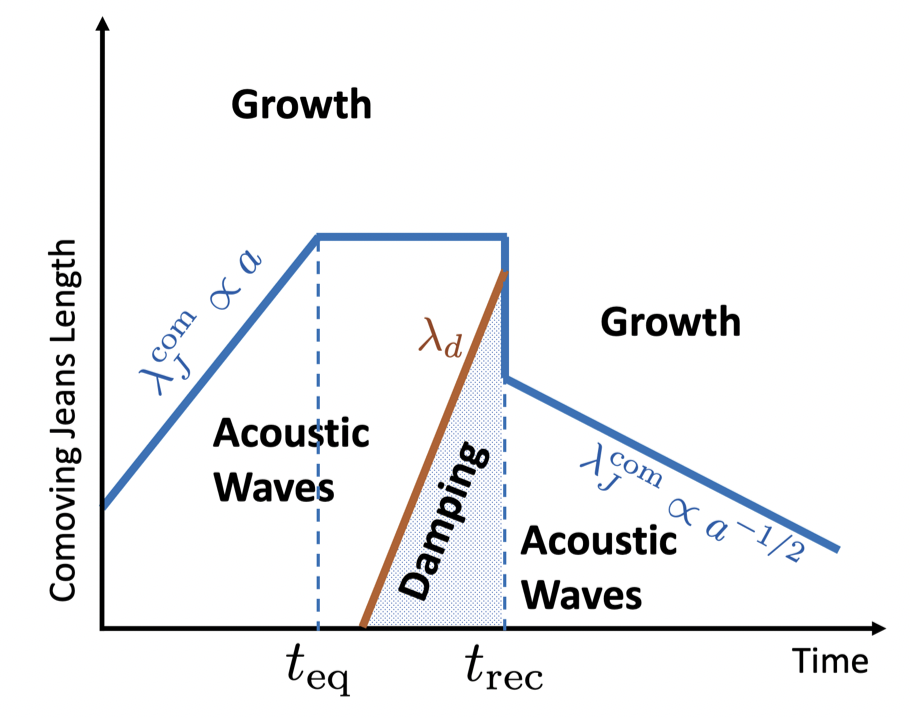
\includegraphics[width=1.0\linewidth]{Jeans_scale.png}
	\caption{共动坐标下金斯长度随时间的变化} \label{Jeans_scale}
\end{figure}

\begin{itemize}
    \item $t>t_\text{rec}$ 时,  $\bar{\rho}\propto a^{-3}$, $c_s\propto a^{-1}$, $\lambda_\text{J}^\text{comoving} \propto a^{-1/2}$.
    \item $t_\text{eq}<t<t_\text{rec}$ 时,  $\bar{\rho}\propto a^{-3}$, $c_s\propto a^{-1/2}$, $\lambda_\text{J}^\text{comoving} \propto a^{0}$, 但存在 Silk Damping.
    \item $t<t_\text{eq}$ 时, $\bar{\rho}\propto a^{-4}$, $c_s\propto a^{0}$, $\lambda_\text{J}^\text{comoving} \propto a$.
\end{itemize}

因为 Silk damping 的存在,到recombination时,所有小尺度的 重子涨落都被擦除,
结构形成只能是大尺度的涨落先涨起来,然后再逐渐过渡到小尺度,这叫做
Top-down Scenario.
但 Top-down Scenario
存在一些问题:
在 Top-down Scenario 中,要形成今天的大尺度结构,需要 recombination 时
的物质涨落 $|\delta_m|> 10^{-3}$. 
而物质涨落和CMB涨落相联系
$\frac{\delta T}{T}=\frac{1}{4} |\delta_r| = \frac{1}{4} \times \frac{4}{3} |\delta_m| \sim 10^{-3}$.
早期CMB的测量就排除了 Top-down Scenario. 今天测量到 CMB涨落约为 
$\frac{\delta T}{T} \sim 10^{-5}$.

可见仅有重子涨落 无法解释现有的观测迹象,需要另一种物质来提供涨落,这就是暗物质。
% \new{冷暗物质可以将金斯质量大大压低,从而解决 Top-down Scenario 的问题。}
% Peebles 等 发展了 新的模型: recombination之前 isothermal perturbation,
% 此时 声速很小,所以金斯尺度也很小, 没有 Silk damping . 金斯mass 1e6 M_sun
%  bottom-up
% CMB涨落还是太大
%  isothermal perturbation un-natural
% 重子的 perturbation 无法解释现有的观测迹象,需要

\subsection{考虑宇宙膨胀}

上节课我们在计算重子物质涨落时忽略宇宙膨胀,现在我们加上这个效应(Hubble drag,下式左边第二项),完整的线性微扰方程为
% 考虑 Hubble drag,(下式左边第二项)
\begin{equation} \label{eq:lin-pertur_Fouri}
    \frac{d^2 \delta_{\vec{k}}}{dt^2 } + 2\frac{\dot{a}}{a} \frac{d\delta_{\vec{k}}}{dt} = \left[4\pi G \bar{\rho}-\frac{k^2c_s^2}{a^2}\right] \delta_{\vec{k}} -\frac{2}{3}\frac{\bar{T}}{a^2}k^2 S_{\vec{k}}
\end{equation}
我们忽略声速项 $\frac{k^2c_s^2}{a^2} \delta_{\vec{k}}$,并且假设 isentropic perturbations, 所以 也忽略 $\frac{2}{3}\frac{\bar{T}}{a^2}k^2 S_{\vec{k}}$. 
线性微扰方程变成
\begin{equation} \label{eq:lin-pertur}
    \frac{d^2 \delta_{\vec{k}}}{dt^2 } + 2\frac{\dot{a}}{a} \frac{d\delta_{\vec{k}}}{dt} = 4\pi G \bar{\rho} \delta_{\vec{k}} 
\end{equation}
% 分两种情况考虑。

在物质为主 ($\Omega_M=1$) 的宇宙里,其增长解由 随时间exp指数增长 减为 随时间幂次增长,
即
\refeq{eq:lin-pertur} 的增长解为
\begin{equation}
    \delta_{+} \propto H(t) \int_{0}^{t} \frac{d t^{\prime}}{a^{2}\left(t^{\prime}\right) H^{2}\left(t^{\prime}\right)} \propto H(z) \int_{z}^{\infty} \frac{1+z^{\prime}}{E^{3}\left(z^{\prime}\right)} d z^{\prime} \propto t^{2/3}
\end{equation}
也就是说,Hubble drag延缓了宇宙物质扰动的增长速度。

在物质主导期($\Omega_M\approx 1$),
\begin{equation}
    \delta_{+}  \propto  t^{2/3} \propto a =\frac{1}{1+z}
\end{equation}

将 $\delta_{\vec{k}}$   的空间部分和时间部分分开: $\delta_{\vec{k}}(t) = \delta_{\vec{k}}(t_0) D(t)$, 其中 定义了 $D(t)$ 是线性增长率(linear growth rate), 写做 红移的函数为 $D(z)=g(z)/(1+z)$.
此时 
\begin{equation}
    \delta_{+} \propto D(t) \propto a =\frac{1}{1+z}
\end{equation}

\reffig{fig:Bary_pert} 总结了考虑宇宙膨胀时的重子涨落情况。

\begin{figure}[!hbtp]
	\centering 
	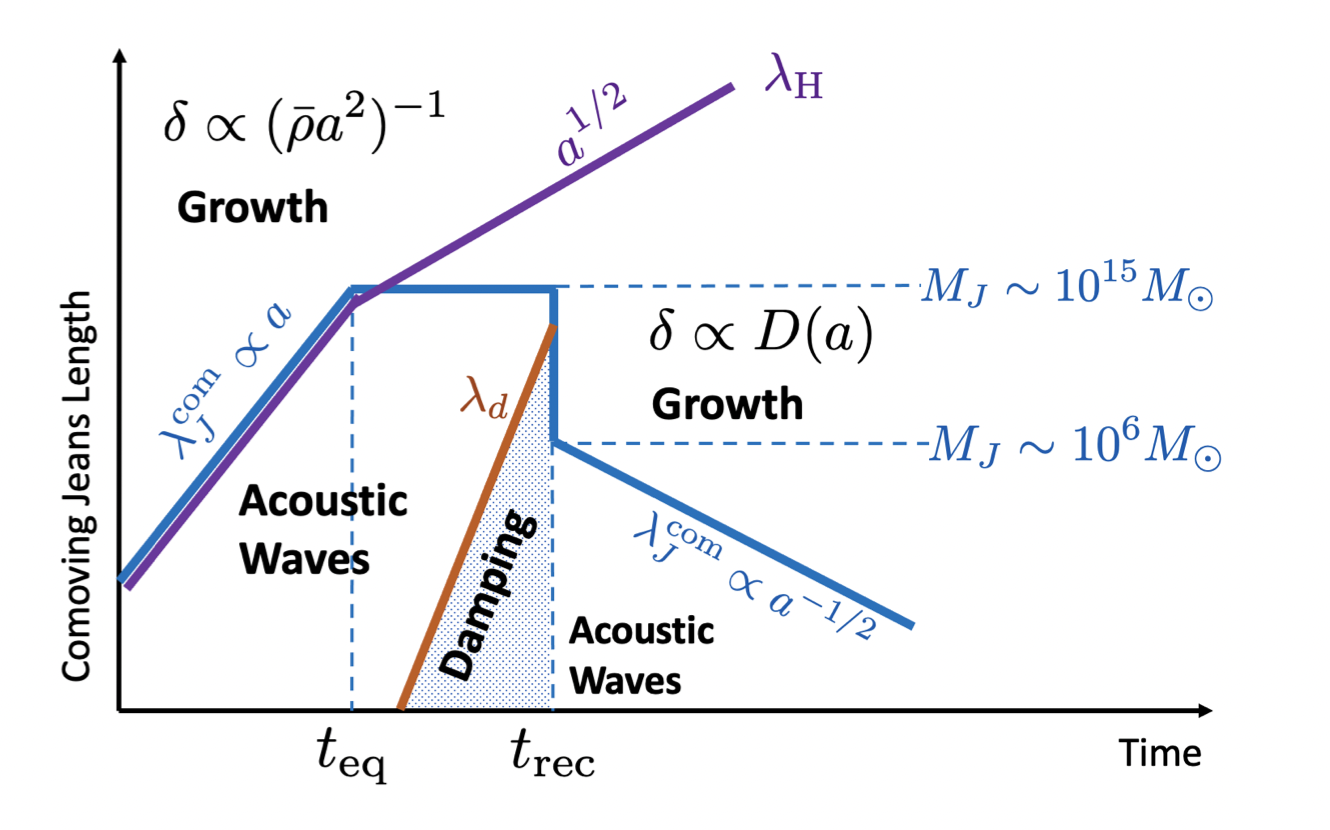
\includegraphics[width=1.0\linewidth]{Baryon_pert_H.png}
	\caption{考虑宇宙膨胀时的重子涨落}
    \label{fig:Bary_pert}
\end{figure}


\end{document}
